% Drawing 73/01-9 -- folder 73, batch 01, archive page 1 (PDF page 2).
% Transcription: plus bas encore, un triangle vu comme hexagone dégénéré : sommets $s_0 = s_1$, $s_2 = s_3$, $s_4 = s_5$, côtés $d_0 = d_1$ (en bas), $d_2 = d_3$ (à droite), $d_4 = d_5$ (à gauche, épaissi).
% Kind: triangle as a degenerate hexagon. Method 2 (schematic redraw from the facsimile). Status: ok.
% Notes: As on the page: the triangle between its three computed vertices, the left side heavy; vertex labels s_0 = s_1, s_2 = s_3, s_4 = s_5; side labels d_4 = d_5, d_2 = d_3, and for the bottom side d_0 with the equality sign written vertically under it and d_1 below. Nothing left out. Redrawn 2026-11-12 (issue 128): to check again.
% Coordinates: 1 unit = 1 mm = 1/100 of the crop width (bbox in page fractions: [0.2, 0.63, 0.44, 0.73]).
% Redrawn by Claude (claude-fable-5-2), issue #128, 2026-11-12; not checked by a human; not compiled (no TeX in the session).
% Rights: reproduces part of the work -- behind RENDER_TRANSCRIPTS, never published by itself.
\documentclass[tikz,border=3pt]{standalone}
\usepackage{amsmath,amssymb}
\usetikzlibrary{patterns,arrows.meta}
\tikzset{pencil/.style={black!45}, struck/.style={black!35}, mpt/.style={circle,draw,inner sep=1.3pt}, pt/.style={circle,fill,inner sep=0.9pt}, opt/.style={circle,draw,fill=white,inner sep=1.1pt}}
\begin{document}
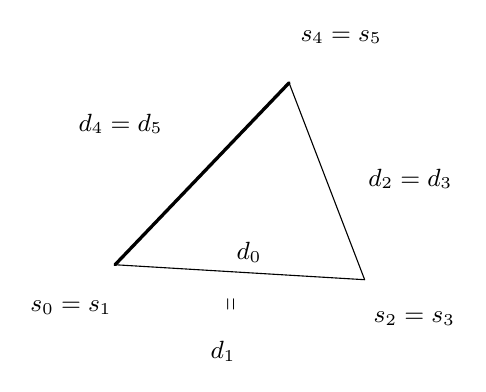
\begin{tikzpicture}[x=1mm,y=1mm,line cap=round,line join=round,font=\scriptsize]
\draw (21,-43) -- (52.7,-44.9) -- (43.1,-19.9);
\draw[very thick] (43.1,-19.9) -- (21,-43);
\node[inner sep=1pt] at (49.7,-14.1) {\small $s_4=s_5$};
\node[inner sep=1pt] at (21.7,-25.1) {\small $d_4=d_5$};
\node[inner sep=1pt] at (58.5,-32.1) {\small $d_2=d_3$};
\node[inner sep=1pt] at (38,-41.4) {\small $d_0$};
\node[inner sep=1pt] at (35.7,-47.9) {\small $\shortparallel$};
\node[inner sep=1pt] at (34.7,-54) {\small $d_1$};
\node[inner sep=1pt] at (15.4,-48.4) {\small $s_0=s_1$};
\node[inner sep=1pt] at (59,-49.8) {\small $s_2=s_3$};
\end{tikzpicture}
\end{document}
